\documentclass[UTF8,a4paper,11pt]{ctexart}
\usepackage{amsmath}
\usepackage{booktabs}
\usepackage{float}
\usepackage{geometry}
\usepackage{graphicx}
\usepackage{hyperref}
\geometry{margin=2.4cm}
\graphicspath{{../figures/}}
\hypersetup{hidelinks,pdfauthor={Anonymous},pdftitle={Curve fitting reproducibility report}}
\title{带噪二维数据的线性拟合与可复现性验证}
\author{匿名}
\date{}

\begin{document}
\maketitle

\begin{abstract}
本文针对一组固定保存的带噪二维合成数据，建立带截距的一元线性最小二乘模型，
通过独立子进程执行求解代码，并以结构化结果驱动图、表与本文生成。
样本数为 36，拟合得到斜率 2.557205、截距 3.133504，
均方根误差为 0.819939，决定系数为 0.988464。
该示例只验证工程闭环，不代表真实竞赛数据或现实规律。
\end{abstract}

\section{问题说明}
给定文件 \texttt{data.csv} 中的观测对 $(x_i,y_i)$，要求估计线性关系，计算误差指标，
分析残差，并生成可追溯的中文报告。输入是固定保存并进行哈希跟踪的 synthetic fixture；
正式运行只读取该文件，不依赖重新生成观测。

\section{模型假设}
\begin{enumerate}
  \item 在给定区间内，响应变量的条件均值可由线性函数近似；
  \item 观测误差均值为零，且本示例不据此主张样本外泛化；
  \item 所有观测在拟合中权重相同，输入文件无缺失值。
\end{enumerate}

\section{符号说明}
\begin{center}
\begin{tabular}{cl}
\toprule
符号 & 含义 \\
\midrule
$x_i$ & 第 $i$ 个自变量观测 \\
$y_i$ & 第 $i$ 个响应变量观测 \\
$\hat y_i$ & 模型预测值 \\
$e_i=y_i-\hat y_i$ & 残差 \\
$a,b$ & 斜率和截距 \\
\bottomrule
\end{tabular}
\end{center}

\section{模型建立}
采用模型
\begin{equation}
  \hat y_i = a x_i + b,
\end{equation}
并最小化残差平方和 $\sum_i(y_i-a x_i-b)^2$。误差指标定义为
\begin{align}
\mathrm{RMSE} &= \sqrt{\frac1n\sum_i e_i^2}, &
\mathrm{MAE} &= \frac1n\sum_i |e_i|, \\
R^2 &= 1-\frac{\sum_i e_i^2}{\sum_i(y_i-\bar y)^2}.
\end{align}

\section{求解方法}
求解程序使用 SciPy 的非线性最小二乘接口估计 $a,b$，但模型本身为线性函数。
Python \texttt{random} 和 NumPy 随机种子均固定为 20260710；求解阶段不重新生成数据。
实际源码、命令、输入哈希、环境摘要、stdout 与 stderr 均保存在当前 run 目录。

\section{结果}
参数估计见表~\ref{tab:parameters}，误差指标见表~\ref{tab:metrics}。
\begin{table}[H]
\centering
\caption{线性模型参数估计}
\label{tab:parameters}
\begin{tabular}{llrl}
\toprule
参数 & 符号 & 原始数值 & 展示数值 \\
\midrule
斜率 & a & 2.5572047133 & 2.557205 \\
截距 & b & 3.1335039092 & 3.133504 \\
\bottomrule
\end{tabular}
\end{table}

\begin{table}[H]
\centering
\caption{拟合误差指标}
\label{tab:metrics}
\begin{tabular}{lrl}
\toprule
指标 & 原始数值 & 展示数值 \\
\midrule
RMSE & 0.8199391781 & 0.819939 \\
MAE & 0.6476007559 & 0.647601 \\
R² & 0.9884643818 & 0.988464 \\
最大绝对误差 & 1.8165114730 & 1.816511 \\
\bottomrule
\end{tabular}
\end{table}


原始观测与拟合曲线见图~\ref{fig:fit}。该图直接读取实际预测结果生成。
\begin{figure}[H]
  \centering
  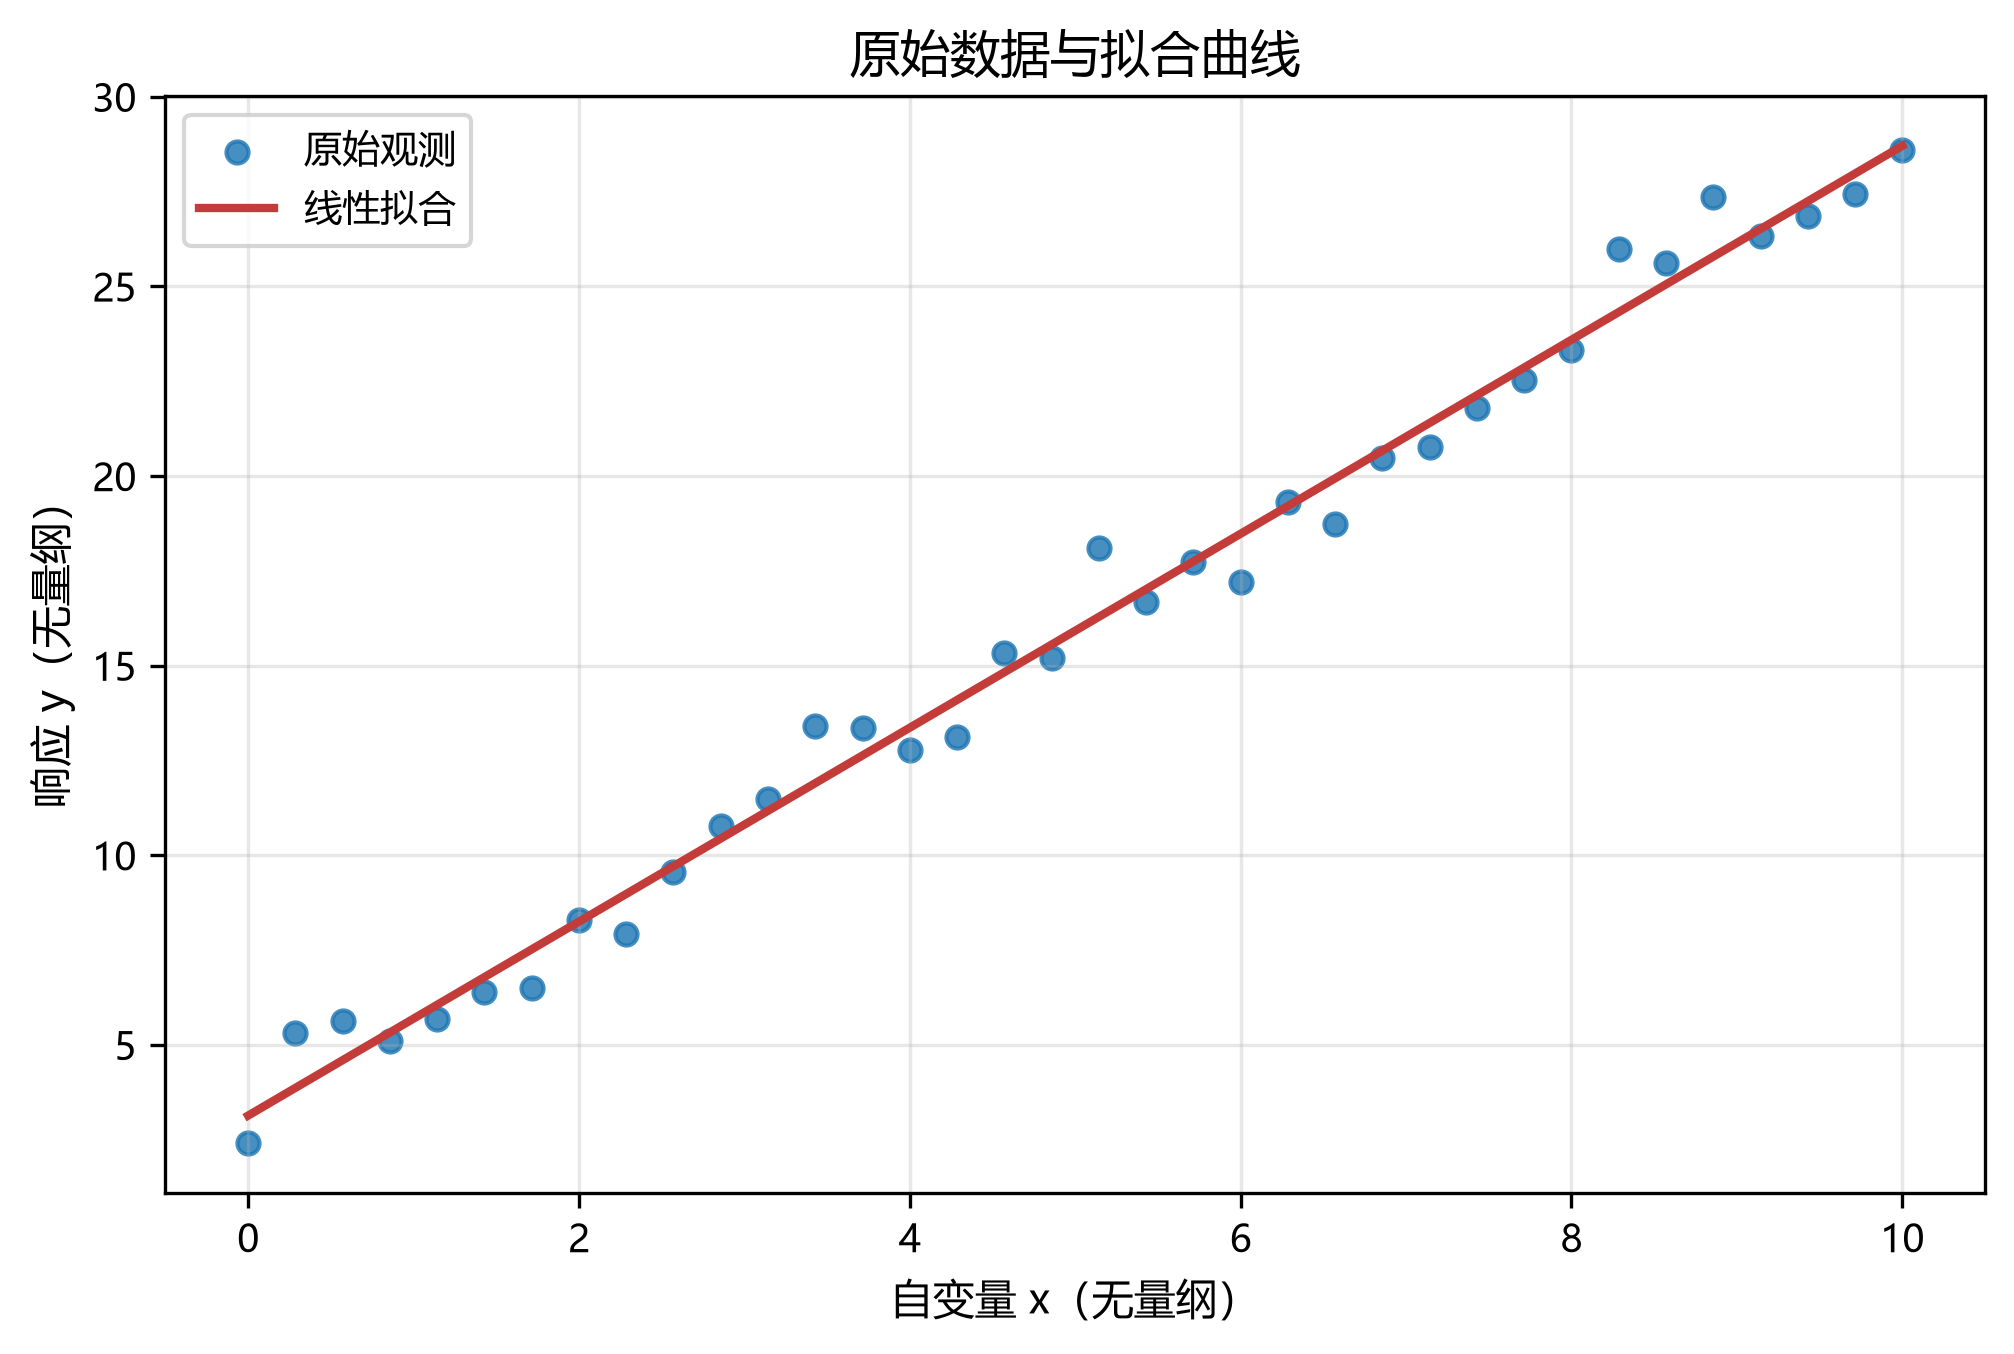
\includegraphics[width=0.86\textwidth]{fit_curve.png}
  \caption{原始数据与实际拟合曲线}
  \label{fig:fit}
\end{figure}

\section{误差分析}
本次运行的 MAE 为 0.647601，最大绝对误差为 1.816511。
独立验证器计算的残差均值为 -2.060e-15，在容差范围内接近零。
图~\ref{fig:residuals} 给出残差随 $x$ 的变化；图中未见需要在本工程 fixture 中进一步建模的明显单调趋势，
但该视觉判断不构成同方差、独立性或样本外泛化的统计检验。
\begin{figure}[H]
  \centering
  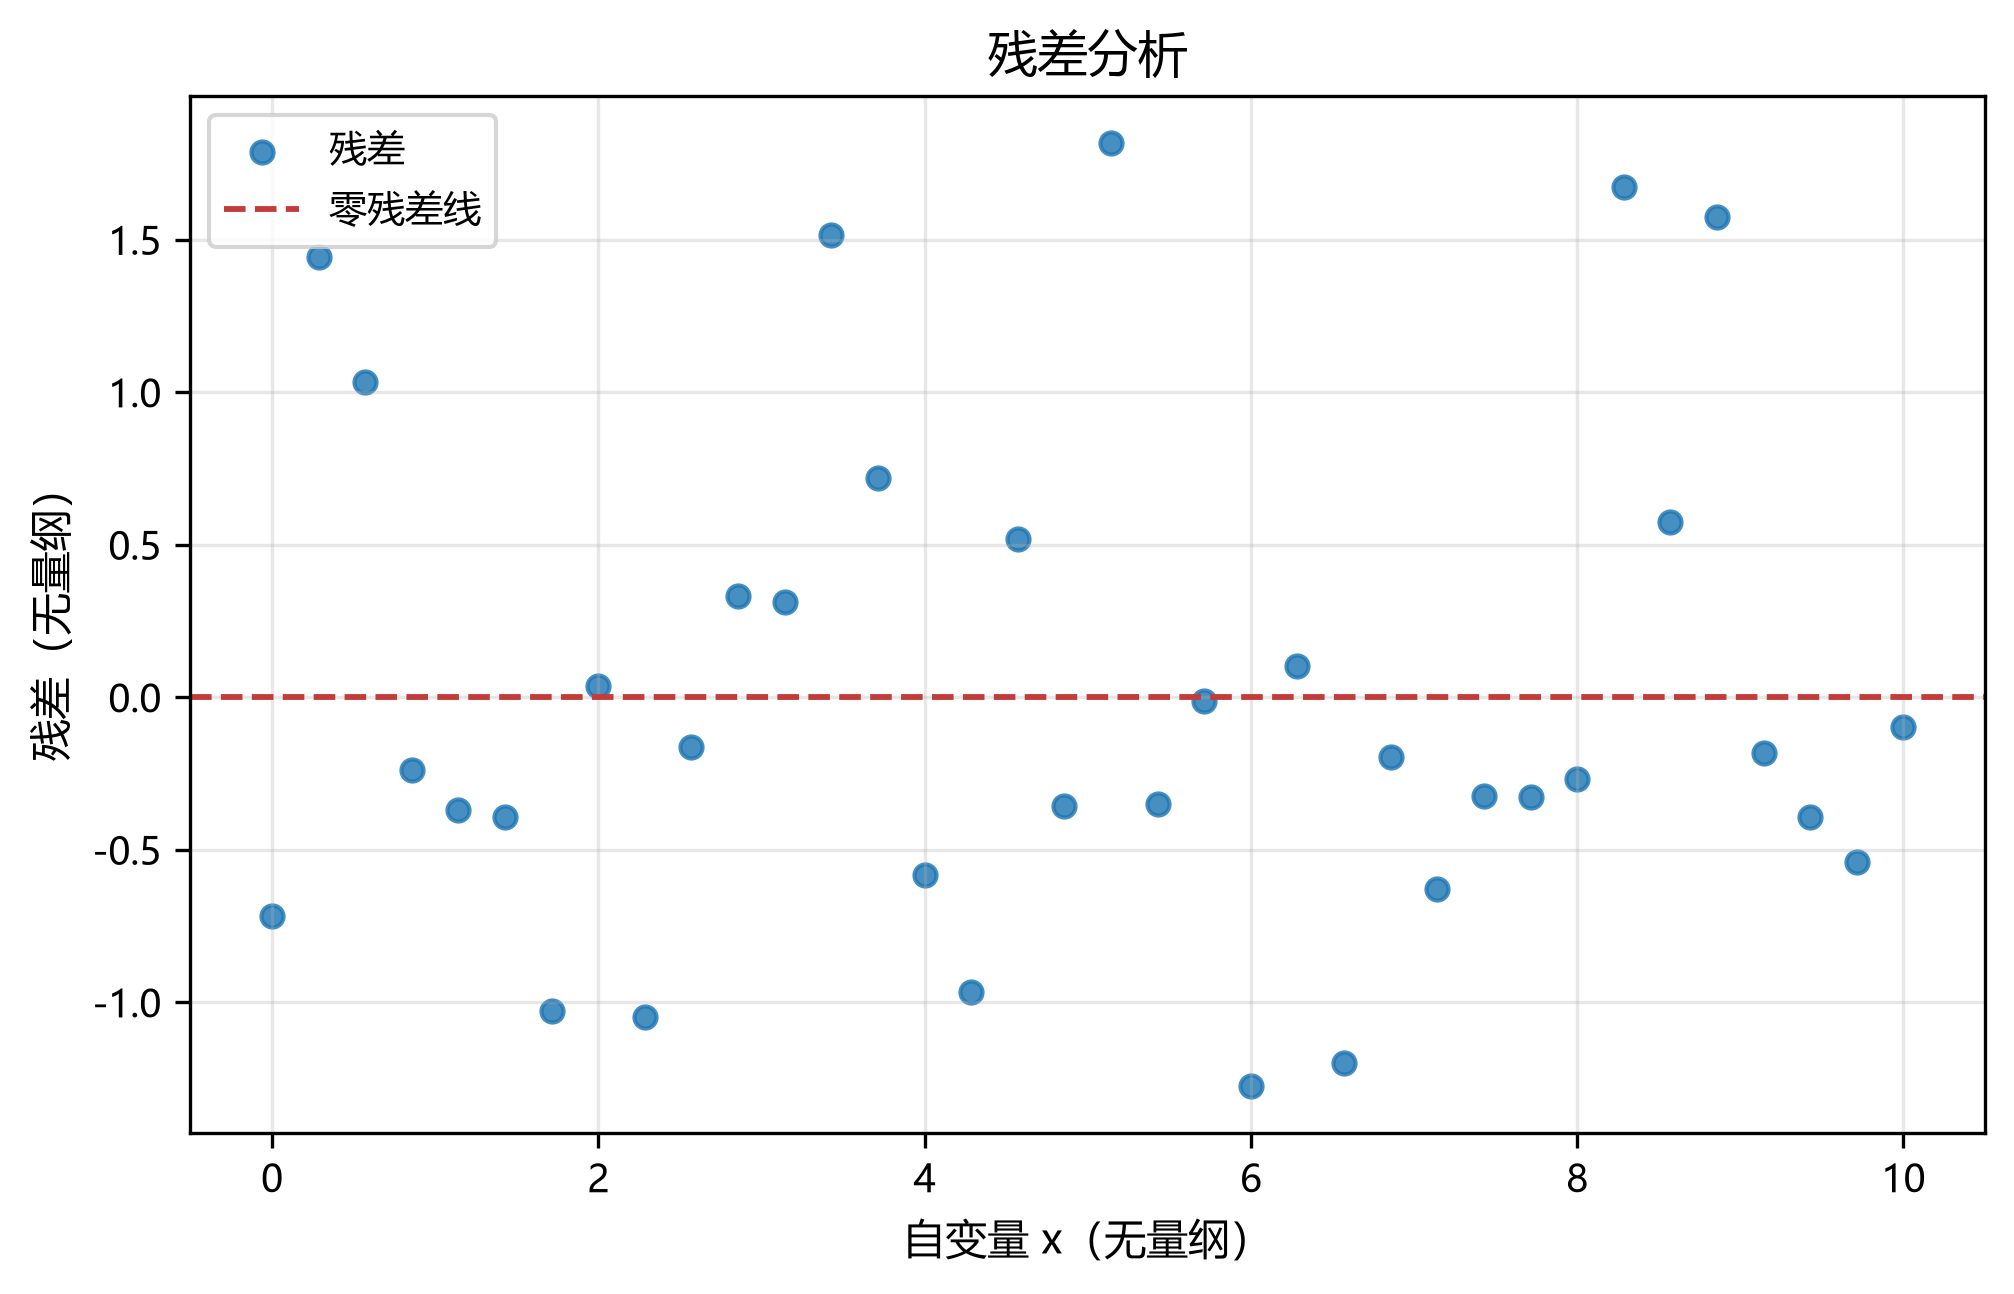
\includegraphics[width=0.86\textwidth]{residuals.png}
  \caption{残差分布}
  \label{fig:residuals}
\end{figure}

\section{结论}
在这组固定合成数据上，线性模型取得 RMSE=0.819939、MAE=0.647601、
$R^2$=0.988464。这些数字来自 \texttt{metrics.json}，不是手工填入的独立结论。
数据规模和生成机制限制了结论范围，因此结果只用于验证 MathModelAgent 的可执行闭环。

\section{复现说明}
复现运行保留固定输入、正式源码、配置和随机种子，并在隔离目录中重新执行各阶段。
复现报告按浮点容差比较参数、指标、预测值和图表源数据，
同时单独记录可能由元数据造成的 PNG、SVG 或 PDF 二进制差异。

\end{document}
